% Credence Development Log -- a companion seminar
%
% Style note: this deck deliberately matches tutorial/tutorial.tex (metropolis,
% 16:9, accent #4A9EFF) so it reads as a companion to the Module 5 tutorial rather
% than a separate document. The extended palette (slate / navorange / resultgreen /
% softgray) is taken from the instats seminar preamble used by the workshop modules,
% and the orange/green match the app's own CSS variables.
%
% Build:  latexmk -pdf devlog.tex     (from this folder)

\documentclass[aspectratio=169]{beamer}

% Theme and packages
\usetheme{metropolis}
\usepackage[utf8]{inputenc}
\usepackage{amsmath, amssymb, mathtools, bm}
\usepackage{graphicx}
\usepackage{booktabs}
\usepackage{lmodern}
\usefonttheme{professionalfonts}
\usepackage{microtype}
\usepackage{xcolor}
\usepackage{hyperref}
\usepackage[absolute,overlay]{textpos}
\usepackage{tikz}
\usetikzlibrary{positioning,arrows.meta,shapes.geometric,calc}

\title[Credence dev log]{Building the Credence Capability}
\subtitle{A development log that doubles as a seminar}
\author{Andy Wilson \enskip\textbar\enskip wilson.stats@gmail.com}
\institute{}
\date{}

\definecolor{accent}{HTML}{4A9EFF}
\definecolor{slate}{HTML}{23373B}
\definecolor{navorange}{HTML}{FD7E14}
\definecolor{resultgreen}{HTML}{1C8B4A}
\definecolor{softgray}{HTML}{F3F6F7}
\definecolor{alertred}{HTML}{DC3545}

\setbeamercolor{structure}{fg=accent}
\setbeamercolor{background canvas}{bg=white}
\setbeamercolor{alerted text}{fg=accent}
\setbeamerfont{frametitle}{series=\bfseries}
\metroset{progressbar=frametitle,block=fill}
\setbeamertemplate{navigation symbols}{}
\setbeamertemplate{footline}{}

\hypersetup{colorlinks=true, urlcolor=accent, linkcolor=accent}

% A compact "what this bought us" stamp, used to close each dev-log entry.
\newcommand{\payoff}[1]{%
  \vspace{0.4em}
  \begin{tikzpicture}
    \node[draw=resultgreen!60, fill=resultgreen!7, rounded corners=2pt,
          text width=0.93\textwidth, align=left, inner sep=7pt]
      {\small\color{slate}\textbf{Why it matters:} #1};
  \end{tikzpicture}}

% The same, in the register of "this is what we got wrong".
\newcommand{\defectbox}[1]{%
  \vspace{0.4em}
  \begin{tikzpicture}
    \node[draw=navorange!60, fill=navorange!7, rounded corners=2pt,
          text width=0.93\textwidth, align=left, inner sep=7pt]
      {\small\color{slate}\textbf{The defect:} #1};
  \end{tikzpicture}}

\begin{document}

% Title slide
\begin{frame}[plain]
  \titlepage
\end{frame}

% ----------------------------------------
\begin{frame}{What this document is}
  \small
  A running record of how the Credence teaching app is being extended --- written
  as a seminar rather than as changelog entries, because most of what we learned is
  worth teaching.

  \vspace{0.6em}
  \textbf{Three threads run through it:}
  \begin{enumerate}
    \item \textbf{The Credence framework} --- what it does, and the boundary between
          \emph{realism} and \emph{truth} that makes it work.
    \item \textbf{The road to CausalMix} --- where a hand-rolled conditional VAE runs
          out of road, argued from defects we actually hit rather than from the abstract.
    \item \textbf{\texttt{survcausal-pilot}} --- the larger project this feeds. Every
          entry closes by saying what it bought \emph{there}, not just here.
  \end{enumerate}

  \vspace{0.6em}
  \textcolor{accent}{\textbf{Companion to:}} \texttt{tutorial/tutorial.pdf}
  (Module 5, instats SSC 2026).
\end{frame}

% ----------------------------------------
\begin{frame}{Roadmap}
  \small
  \begin{columns}[T,totalwidth=\textwidth]
    \begin{column}{0.48\textwidth}
      \textbf{Part I --- The framework}\\
      Realism vs.\ truth; why the split matters.
      \vspace{0.5em}

      \textbf{Part II --- Tier 0: making the claims true}\\
      Six defects, one of which was found \emph{by} the fix for another.
      \vspace{0.5em}

      \textbf{Part III --- Toward CausalMix}\\
      Post-hoc repair vs.\ architectural fix.
    \end{column}
    \begin{column}{0.48\textwidth}
      \textbf{Part IV --- \texttt{survcausal-pilot}}\\
      The larger project: what it is, what it still needs, and how this work
      supplies it.
      \vspace{0.5em}

      \textbf{Part V --- Tier 1}\\
      $\tau(X)$ heterogeneity, an overlap dial, and factorial scenarios.
    \end{column}
  \end{columns}
\end{frame}

% ========================================
\section{Part I --- The framework}
% ========================================

\begin{frame}{The problem Credence solves}
  \small
  You have an estimator. Does it work on \emph{your} data? You cannot tell, because
  the individual causal effect is never observed. So the field validates on
  simulation --- and simulation has its own problem:

  \begin{itemize}
    \item we hand-specify the data-generating process;
    \item a hand-specified DGP embeds parametric assumptions;
    \item those assumptions may quietly \textbf{favour some estimators over others}.
  \end{itemize}

  Credence (Parikh et al., ICML 2022) separates the two things a benchmark needs:

  \begin{center}
  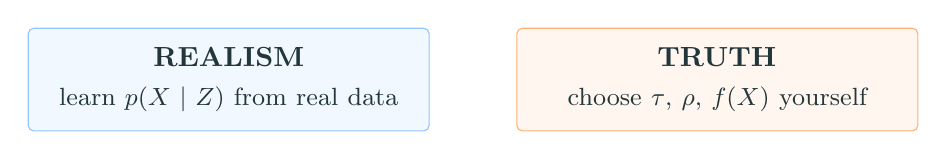
\begin{tikzpicture}[node distance=0.7cm]
    \node[draw=accent!60, fill=accent!7, rounded corners=2pt, text width=4.6cm,
          align=center, inner sep=7pt] (r)
      {\color{slate}\textbf{REALISM}\\[2pt]\small learn $p(X\mid Z)$ from real data};
    \node[draw=navorange!60, fill=navorange!7, rounded corners=2pt, text width=4.6cm,
          align=center, inner sep=7pt, right=1.1cm of r] (t)
      {\color{slate}\textbf{TRUTH}\\[2pt]\small choose $\tau$, $\rho$, $f(X)$ yourself};
  \end{tikzpicture}
  \end{center}

  \vspace{0.3em}
  \textcolor{accent}{\textbf{The trick:}} because \emph{you} chose $\tau$, you can score
  any estimator. Because the covariates came from real data, the benchmark is not a
  toy.
\end{frame}

% ----------------------------------------
\begin{frame}{The boundary that has to hold}
  \small
  The generator learns $p(X \mid Z)$ and \textbf{never sees the outcome}.

  \vspace{0.5em}
  This is not a detail. If the generator knew the treatment effect, then
  ``recovering'' that effect downstream would prove nothing --- you would be
  measuring how well information flows through your own pipeline, not whether an
  estimator works.

  \vspace{0.6em}
  In the code, that boundary is a file boundary:
  \begin{itemize}
    \item \texttt{cvae\_model.py} --- realism. No $Y$, no $\tau$, anywhere in it.
    \item \texttt{dgp.py} --- truth. Chooses $\tau$, $\rho$, $f(X)$.
    \item \texttt{realism.py} --- evidence. Checks the first one actually worked.
  \end{itemize}

  \payoff{Keeping realism and truth in separate files makes the boundary auditable.
  A reviewer can confirm the generator never touches $Y$ by reading one import list.}
\end{frame}

% ----------------------------------------
\begin{frame}{The generative order looks backwards (and is fine)}
  \small
  In the world, $X$ causes $Z$: sicker patients are treated differently.
  In the app we draw $Z$ first, then $X \mid Z$.

  \vspace{0.5em}
  That is not an error. $p(X,Z) = p(Z)\,p(X\mid Z)$ is a valid factorization of the
  same joint distribution --- we are \emph{sampling from the joint}, not asserting a
  causal direction. A conditional VAE finds $p(X \mid Z)$ far easier to learn than
  the reverse.

  \vspace{0.6em}
  \textbf{What it does cost us:} the \emph{strength} of observed confounding is
  inherited from whatever the real data happened to contain. It is not a dial.

  \vspace{0.4em}
  Making it a dial --- along with overlap --- is exactly what Part V is about.
\end{frame}

% ========================================
\section{Part II --- Tier 0: making the claims true}
% ========================================

\begin{frame}{Where we started}
  \small
  The app told users its output was
  \textit{``realistic and near-indistinguishable from the observed sample.''}

  \vspace{0.6em}
  It never checked. And underneath the claim were six defects.

  \vspace{0.5em}
  \begin{center}
  \small
  \begin{tabular}{@{}ll@{}}
    \toprule
    \textbf{What was wrong} & \textbf{Consequence} \\
    \midrule
    One gradient step per epoch      & generator barely trained \\
    Decoder round-trip never called  & export did not match your schema \\
    $f(X)$ selected columns by name  & snake\_case covariates silently dropped \\
    $f(X)$ averaged on raw scale     & dollars drowned out years \\
    No seed on generation            & nothing reproducible \\
    No realism check at all          & the headline claim was unfalsifiable \\
    \bottomrule
  \end{tabular}
  \end{center}

  \vspace{0.5em}
  \textcolor{accent}{\textbf{The through-line:}} an app that asserts its own quality
  without evidence is precisely the thing Module E trains participants to catch.
\end{frame}

% ----------------------------------------
\begin{frame}{Defect 1 --- fifty gradient steps}
  \small
  The training loop called \texttt{optimizer.step()} \textbf{once per epoch}, on the
  whole dataset at once. At the app's default of 50 epochs, that is
  \textbf{50 gradient steps in total}.

  \defectbox{The ``learned covariate structure'' was closer to the untrained prior
  than to the data --- while the interface promised near-indistinguishability.}

  \vspace{0.4em}
  \textbf{Fixed:} minibatching, with $\lceil n/\text{batch}\rceil$ steps per epoch, a
  seeded shuffle, and a per-observation ELBO so the reported number means the same
  thing at any batch size.

  \vspace{0.3em}
  {\footnotesize Measured, pneumonia cohort, 5 epochs: full-batch $=1$ step/epoch,
  $-$ELBO $3.62$; minibatch(128) $=8$ steps/epoch, $-$ELBO $\mathbf{2.93}$.}

  \payoff{We kept ``Full dataset (the old bug)'' as a menu option, so the workshop can
  \emph{reproduce} the failure and watch the realism score degrade --- rather than
  take our word for it.}
\end{frame}

% ----------------------------------------
\begin{frame}{The fix that mattered most --- measuring realism}
  \small
  Three checks, weakest to strongest, all against \textbf{held-out rows the generator
  never trained on}:

  \vspace{0.5em}
  \begin{center}
  \small
  \begin{tabular}{@{}lll@{}}
    \toprule
    \textbf{Check} & \textbf{Question} & \textbf{Catches} \\
    \midrule
    SMD                & are the means close?          & location \\
    KS distance        & are the \emph{distributions} close? & spread, skew, modes \\
    Discriminator AUC  & can a model tell them apart?  & broken \emph{correlations} \\
    \bottomrule
  \end{tabular}
  \end{center}

  \vspace{0.6em}
  \textbf{Why all three.} A generator can match every marginal mean and get every
  shape wrong. It can match every marginal distribution and still destroy the
  \emph{joint} structure --- and only the discriminator, which sees whole rows, can
  notice that.

  \vspace{0.5em}
  \textcolor{accent}{\textbf{AUC $\approx 0.5$ is the target.}} This is the rare model
  you want to perform badly. Participants find that disorienting, which makes it stick.
\end{frame}

% ----------------------------------------
\begin{frame}{Why the holdout is not optional}
  \small
  These metrics must compare synthetic data against real rows the generator has
  \textbf{never seen}.

  \vspace{0.6em}
  Scored against its own training rows, a flexible generator wins by
  \textbf{memorising}. That is:
  \begin{itemize}
    \item a meaningless result --- it says nothing about generalisation; and
    \item a \textbf{privacy problem} --- a generator that memorises patients can leak
          them, and participants upload their own files.
  \end{itemize}

  \vspace{0.5em}
  So Step 2 now splits before it trains, and Step 4 compares against the holdout.

  \payoff{Privacy metrics are one of the things CausalMix ships and we do not. The
  holdout is the minimum honest version of that idea.}
\end{frame}

% ----------------------------------------
\begin{frame}{Defect 10 --- the diagnostic found a bug we had not listed}
  \small
  First run of the new realism check, after 150 epochs of proper training:

  \begin{center}
    \color{alertred}\textbf{\Large Discriminator AUC = 1.000}
  \end{center}

  Perfect separation. The obvious reading --- ``the generator is hopeless'' --- was wrong.

  \vspace{0.3em}
  \begin{center}
  \footnotesize
  \begin{tabular}{@{}lll@{}}
    \toprule
    \textbf{Covariate} & \textbf{Real} & \textbf{Synthetic} \\
    \midrule
    \texttt{priorPneumonia} & $\{0, 1\}$ & $[-0.30,\ 1.35]$ continuous \\
    \texttt{priorVaccine}   & $\{0, 1\}$ & $[-0.25,\ 1.35]$ continuous \\
    \bottomrule
  \end{tabular}
  \end{center}

  The decoder round-trip only ever handled \texttt{object}/\texttt{Categorical}
  columns. \textbf{Binary and integer covariates were exported as continuous
  relaxations.} The classifier was not detecting anything subtle --- it was asking
  ``is this value exactly 0 or 1?''

  \payoff{The diagnostic paid for itself on its first run --- by finding a defect
  that was not on the list it was built to check.}
\end{frame}

% ----------------------------------------
\begin{frame}{Sampling, not rounding}
  \small
  Fixing it raises a genuine statistical choice. Given decoder output implying
  $P = (0.62, 0.31, 0.07)$ across three categories:

  \vspace{0.5em}
  \begin{columns}[T,totalwidth=\textwidth]
    \begin{column}{0.47\textwidth}
      \textbf{argmax / threshold}\\
      Always take the most likely.
      \begin{itemize}
        \item every row $\to$ category 1
        \item rare categories \textbf{vanish}
        \item synthetic data less variable than real
      \end{itemize}
    \end{column}
    \begin{column}{0.47\textwidth}
      \textbf{sample}\\
      Draw with those probabilities.
      \begin{itemize}
        \item frequencies come out right
        \item marginal distribution preserved
        \item costs nothing
      \end{itemize}
    \end{column}
  \end{columns}

  \vspace{0.6em}
  What we need to preserve is the \textbf{marginal distribution}, not the most likely
  value of any single row. So we sample --- categorically for categories, Bernoulli
  for binaries, round-and-clip for integers.

  \vspace{0.4em}
  \small Measured: with a true rare-level share of 15\%, sampling returned
  \textbf{16.7\%}; argmax returned \textbf{0\%}.
\end{frame}

% ----------------------------------------
\begin{frame}{Defect 4 and 5 --- what $f(X)$ was}
  \small
  $f(X)$ is the prognostic index: how covariates move $Y(0)$. It \emph{is} the
  observed-confounding mechanism. It was one line:

  \vspace{0.2em}
  {\footnotesize
  \texttt{numeric = [i for i, name in enumerate(names) if '\_' not in name]}\\
  \texttt{hX = X[:, numeric].mean(axis=1)}}

  \vspace{0.3em}
  \textbf{Two independent defects.}
  \begin{enumerate}
    \item \textbf{Selection by name} --- keeps columns whose name has no underscore.
          Meant to skip one-hot dummies; also drops any covariate named
          \texttt{prior\_vaccine}. Still \emph{exported}, so it looked like a
          confounder and influenced nothing.
    \item \textbf{Raw-scale averaging} --- an unweighted mean across units is decided
          by whichever column has the biggest numbers.
  \end{enumerate}

  \payoff{Both built-in datasets use names without underscores --- so it survived.
  The first participant to upload their own file would have hit it.}
\end{frame}

% ----------------------------------------
\begin{frame}{\dots\ and what $f(X)$ is now}
  \small
  Every encoded column participates --- selection by \emph{name} is gone. Each is
  standardised on the \textbf{training} statistics, weighted, and rescaled to a
  stated magnitude:

  \[
    f(X) \;=\; c \cdot \sigma_Y \cdot
    \frac{\sum_j w_j \, z_j}{s},
    \qquad z_j = \frac{x_j - \bar{x}_j}{\mathrm{sd}_j}
  \]

  \begin{itemize}
    \item \textbf{unit-invariant} --- rescale earnings and $f(X)$ does not move;
    \item \textbf{weights visible in the UI} --- weight 0 means cannot confound;
    \item \textbf{magnitude interpretable} --- $c$ is in outcome standard deviations.
  \end{itemize}

  \payoff{Direction is a stated choice ($w$); magnitude is a stated parameter ($c$).
  Turning $c$ into a dial is Tier 1.}
\end{frame}

% ----------------------------------------
\begin{frame}{The property that makes a benchmark usable}
  \small
  \textbf{The exported covariates must fully determine the potential outcomes}
  (up to $U$ and noise).

  \vspace{0.5em}
  If the outcome secretly depends on something we did not export, then \emph{no}
  analyst can adjust for it, \emph{every} estimator looks biased --- and the workshop
  teaches a false lesson about the methods instead of a true one about the data.

  \vspace{0.6em}
  This forced a step the old pipeline did not have:

  \begin{center}
  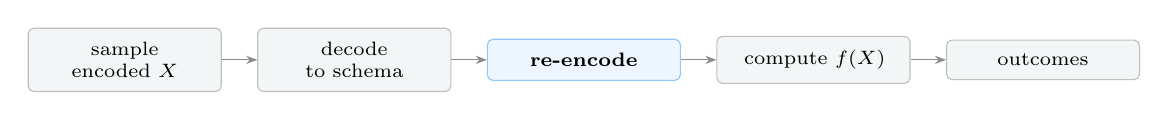
\begin{tikzpicture}[node distance=0.45cm, every node/.style={font=\scriptsize}]
    \node[draw=black!25, fill=softgray, rounded corners=2pt, text width=2.1cm,
          align=center, inner sep=5pt] (a) {sample\\encoded $X$};
    \node[draw=black!25, fill=softgray, rounded corners=2pt, text width=2.1cm,
          align=center, inner sep=5pt, right=of a] (b) {decode\\to schema};
    \node[draw=accent!60, fill=accent!10, rounded corners=2pt, text width=2.1cm,
          align=center, inner sep=5pt, right=of b] (c) {\textbf{re-encode}};
    \node[draw=black!25, fill=softgray, rounded corners=2pt, text width=2.1cm,
          align=center, inner sep=5pt, right=of c] (d) {compute $f(X)$};
    \node[draw=black!25, fill=softgray, rounded corners=2pt, text width=2.1cm,
          align=center, inner sep=5pt, right=of d] (e) {outcomes};
    \draw[-{Stealth[length=4pt]}, black!45] (a)--(b);
    \draw[-{Stealth[length=4pt]}, black!45] (b)--(c);
    \draw[-{Stealth[length=4pt]}, black!45] (c)--(d);
    \draw[-{Stealth[length=4pt]}, black!45] (d)--(e);
  \end{tikzpicture}
  \end{center}

  \vspace{0.3em}
  Without the re-encode, a categorical's \emph{exported} value only loosely tracks the
  value that actually drove the outcome.
\end{frame}

% ----------------------------------------
\begin{frame}{Two seeds, on purpose}
  \small
  Generation used unseeded draws: every click produced different data and nothing was
  reproducible.

  \vspace{0.5em}
  The fix is not one seed but \textbf{two} --- training and generation, kept apart:
  \begin{itemize}
    \item redraw a cohort \emph{without} retraining the model;
    \item retrain \emph{without} moving the cohort;
    \item so you always know which change caused what you are looking at.
  \end{itemize}

  \vspace{0.5em}
  This mirrors \texttt{survcausal-pilot}'s own convention, which seeds the cohort draw
  and the estimator fits from \textbf{disjoint streams} for exactly this reason
  (\texttt{sseed} / \texttt{eseed} in \texttt{run\_pilot.R}).

  \payoff{Attribution. The same principle as the pilot's factorial design: move one
  thing at a time, so any difference has a single cause.}
\end{frame}

% ----------------------------------------
\begin{frame}{The gate: what we refuse to ship without}
  \small
  Ten checks, runnable with \texttt{python3 tests/test\_tier0.py} --- no pytest, so a
  participant can run it on a workshop laptop. The one that matters most:

  \textbf{The truth gate.} With $\rho = 0$ the only path from $Z$ to $Y$ other than the
  effect runs through the exported covariates. A correctly specified adjustment
  \emph{must} recover $\tau$.

  \begin{center}
  \footnotesize
  \begin{tabular}{@{}lrr@{}}
    \toprule
    & \textbf{estimate} & \textbf{bias} \\
    \midrule
    true $\tau$                    & $-5.000$ & --- \\
    naive difference               & $-4.349$ & $+0.651$ \\
    g-computation                  & $\mathbf{-4.977}$ & $\mathbf{+0.023}$ \\
    \bottomrule
  \end{tabular}
  \end{center}
  \vspace{0.1em}
  {\footnotesize (tolerance $\pm 0.130$, four Monte Carlo standard errors)}

  \textbf{Its complement.} At $\rho = 0.8$: adjusting for $X$ leaves bias $+0.284$;
  adding $U$ brings it to $-0.015$.

  \payoff{If the truth gate fails, the generator is wrong and nothing downstream
  can be trusted.}
\end{frame}

% ----------------------------------------
\begin{frame}{Tier 0 --- result}
  \small
  \begin{center}
  \begin{tabular}{@{}lcc@{}}
    \toprule
    \textbf{Discriminator AUC} & \textbf{before} & \textbf{after} \\
    \midrule
    undertrained generator (1 full-batch epoch) & \multicolumn{2}{c}{$0.852$} \\
    properly trained generator                  & $1.000$ & $\mathbf{0.602}$ \\
    \midrule
    app flow, pneumonia cohort                  & --- & $\mathbf{0.579}$ \\
    \bottomrule
  \end{tabular}
  \end{center}

  \vspace{0.4em}
  \small The $1.000 \to 0.602$ column is the type-aware decoder (defect 10). The
  $0.852$ figure is what an undertrained generator still scores \emph{after} that fix
  --- which is why both numbers are reported: the \textbf{improvement} is the teaching
  artifact, not the absolute level.

  \vspace{0.6em}
  \textbf{Verdict at 0.579:} \textit{``Indistinguishable --- the discriminator is near
  chance.''} The claim the app was already making is now one the app can defend.
\end{frame}

% ========================================
\section{Part III --- Toward CausalMix}
% ========================================

\begin{frame}{What CausalMix is}
  \small
  \textbf{CausalMix} --- Zhang, \textbf{Parikh}, Naimi, Nabi, Kim, Lash
  (arXiv:2603.03587, March 2026).

  \vspace{0.5em}
  A conditional VAE with:
  \begin{itemize}
    \item a \textbf{mixture-of-Gaussians latent prior} --- real covariates are
          multimodal and clustered; a single Gaussian smooths that away;
    \item \textbf{data-type-specific decoders} for continuous, binary and categorical
          columns;
    \item an \textbf{overlap regularizer} shaping the propensity-score distribution;
    \item overlap, confounding strength and effect heterogeneity varied
          \textbf{independently at design time}.
  \end{itemize}

  \vspace{0.6em}
  \textcolor{accent}{\textbf{The decisive fact:}} Harsh Parikh is first author of
  Credence \emph{and} an author of CausalMix. This is not a competing school --- it is
  Credence's own lineage, four years on. Adopting it is a continuation, not a retraction.
\end{frame}

% ----------------------------------------
\begin{frame}{Defect 10, revisited --- the case for typed decoders}
  \small
  Our fix for binary and integer columns is \textbf{post-hoc repair}: the network is
  trained as if every column were continuous, and we discretize its output afterwards.

  \vspace{0.5em}
  \begin{columns}[T,totalwidth=\textwidth]
    \begin{column}{0.47\textwidth}
      \textbf{What we did}\\
      \begin{itemize}
        \item MSE loss on every column
        \item Bernoulli-sample binaries after decoding
        \item round-and-clip integers after decoding
      \end{itemize}
      \vspace{0.3em}
      Works. AUC $1.000 \to 0.602$.
    \end{column}
    \begin{column}{0.47\textwidth}
      \textbf{What it cannot fix}\\
      \begin{itemize}
        \item the \emph{training signal} still treats a 0/1 flag as a continuous target
        \item so the \emph{joint} structure between a binary and a continuous covariate
              is learned only approximately
      \end{itemize}
    \end{column}
  \end{columns}

  \vspace{0.6em}
  The architectural fix is to give the model a per-column likelihood and decode
  each type natively --- which is exactly what CausalMix does.

  \payoff{We can now argue for Tier 2 with a \emph{measured} number rather than an
  appeal to authority. That is a better reason to adopt something.}
\end{frame}

% ----------------------------------------
\begin{frame}{Caveats we are not going to forget}
  \small
  \begin{enumerate}
    \item \textbf{Maturity.} March 2026 preprint, no visible CI, not on PyPI,
          effectively one maintainer. Fine for teaching; pin a commit and validate
          before any number reaches a paper.
    \item \textbf{Deployment weight.} shinyapps.io already strains with \texttt{torch}.
          Mitigation --- correct regardless of backend --- \textbf{ship pre-fit
          generators; let the app only sample}.
    \item \textbf{No survival outcomes.} Neither Credence nor CausalMix does
          time-to-event. For \texttt{survcausal-pilot} that is an integration, not a swap.
    \item \textbf{The parametric assumption moves; it does not vanish.} Realism is
          bought for $p(X, Z)$ only. $f(X)$ and $\tau$ are still ours.
    \item \textbf{Self-flattery risk.} A generator fit on the same data used for the
          benchmark can favour estimators whose inductive bias matches the generator ---
          a VAE's smooth latent structure flatters smooth-function learners.
  \end{enumerate}

  \vspace{0.3em}
  \textcolor{accent}{\textbf{Say caveat 5 out loud in the workshop.}} Credence's entire
  pitch is that hand-specified DGPs may inadvertently favour certain estimators. The
  same critique applies to us.
\end{frame}

% ========================================
\section{Part IV --- \texttt{survcausal-pilot}}
% ========================================

\begin{frame}{The larger project}
  \small
  \texttt{survcausal-pilot} --- a pilot for a causal-estimator extension to Diana
  Shamsutdinova's \texttt{survcompare} package.
  \emph{Shamsutdinova--Shuryak--Yang collaboration.}

  \vspace{0.6em}
  \textbf{Two questions, deliberately not conflated:}
  \begin{columns}[T,totalwidth=\textwidth]
    \begin{column}{0.47\textwidth}
      \textbf{What will happen?}\\
      Prognosis. Ranks patients by risk. Scored on discrimination and calibration.
    \end{column}
    \begin{column}{0.47\textwidth}
      \textbf{What should we do?}\\
      Benefit. Targets the treatment effect. Scored on RMSE against a known
      $\mathrm{ATE}(t)$.
    \end{column}
  \end{columns}

  \vspace{0.6em}
  A patient can be high-risk and gain little; lower-risk and gain a lot. A purely
  predictive model conflates the two.

  \vspace{0.4em}
  \textcolor{accent}{\textbf{The causal question needs known truth}} --- which only
  simulation can give. That is where this work connects.
\end{frame}

% ----------------------------------------
\begin{frame}{The pilot's headline result}
  \small
  A $2\times2$ factorial Monte Carlo (50 replicates/cell), crossing confounding shape
  with hazard shape \emph{at a single fixed effect size}, so any difference has one cause.

  \vspace{0.4em}
  \begin{center}
  \small
  \begin{tabular}{@{}lcccc@{}}
    \toprule
    \textbf{relative RMSE} & Cox-PH & RSF & CSF & CAST (spline) \\
    \midrule
    Linear / PH            & \textbf{0.087} & 0.365 & 0.230 & 0.224 \\
    Linear / non-PH        & 0.897 & 0.611 & 0.358 & \textbf{0.352} \\
    Nonlinear / PH         & 0.466 & 0.452 & 0.186 & 0.180 \\
    Nonlinear / non-PH     & 1.148 & 0.764 & 0.250 & \textbf{0.239} \\
    \bottomrule
  \end{tabular}
  \end{center}

  \vspace{0.5em}
  Under simple confounding with proportional hazards a correctly specified Cox model
  wins outright and causal forests add nothing. Break \emph{either} assumption and the
  parametric methods collapse while CSF and CAST hold.

  \vspace{0.4em}
  \textcolor{accent}{\textbf{The lesson:}} the right method is data-dependent. A
  benchmark reporting one regime would mislead.
\end{frame}

% ----------------------------------------
\begin{frame}{What the pilot says it still needs}
  \small
  From the pilot's own vignette and README --- these are not our inventions:

  \vspace{0.5em}
  \begin{itemize}
    \item \textit{``a data-generating process with genuine \textbf{covariate-driven
          effect modification}''} --- named as a natural extension;
    \item \textit{``A future data-generating process can add genuine covariate-level
          heterogeneity; the machinery here would estimate it unchanged''};
    \item \textit{``\textbf{Causal scoring needs known truth.} RMSE against the true
          $\mathrm{ATE}(t)$ is only possible in simulation, which is why the package
          ships simulation DGPs with a treatment arm and oracle effect.''}
  \end{itemize}

  \vspace{0.6em}
  So the pilot's causal-validation story rests entirely on \textbf{simulated DGPs with
  oracle truth} --- and its one soft spot is that those DGPs are hand-specified, in
  exactly the manner Credence was written to criticise.

  \vspace{0.4em}
  \textcolor{accent}{\textbf{A reviewer will ask.}}
\end{frame}

% ----------------------------------------
\begin{frame}{Connection 1 --- $\tau(X)$ is the pilot's named gap}
  \small
  The pilot's risk/benefit quadrants (Figure 3) make their point via a
  \emph{non-monotone} relation between risk and benefit, because the treatment hazard
  ratio depends only on time --- there is \textbf{no covariate-driven effect
  modification} in the cohort. The vignette concedes this twice.

  \vspace{0.6em}
  Tier 1's $\tau(X)$ knob is a prototype of exactly that missing DGP feature.

  \vspace{0.5em}
  \begin{center}
  \small
  \begin{tabular}{@{}lll@{}}
    \toprule
     & \textbf{app (Python)} & \textbf{pilot (R)} \\
    \midrule
    cost of one run   & seconds        & 1--1.5 hours \\
    feedback loop     & immediate      & overnight \\
    stakes            & teaching       & publishable numbers \\
    \bottomrule
  \end{tabular}
  \end{center}

  \payoff{Prototype $\tau(X)$ where a run costs seconds; port it where a run costs
  ninety minutes. The app is the cheap end of the same question.}
\end{frame}

% ----------------------------------------
\begin{frame}{Connection 2 --- the overlap dial feeds a dormant diagnostic}
  \small
  The pilot \emph{already computes} positivity diagnostics: \texttt{pct\_extreme} and
  \texttt{pct\_clipped} in \texttt{run\_causal()}, carried through into the summary table.

  \vspace{0.5em}
  But nothing in the study ever \textbf{varies} overlap. So across all four design
  cells those columns read:

  \begin{center}
    \texttt{0.00000,\quad 0.00000,\quad 0.00036,\quad 0.00047}
  \end{center}

  \vspace{0.5em}
  A diagnostic that never moves is a diagnostic that teaches nothing.

  \vspace{0.5em}
  Tier 1's overlap slider turns a passive column into a \textbf{third design lever} ---
  and it is the axis most likely to separate doubly-robust CSF from the plug-in
  learners in a way non-proportionality alone does not.

  \payoff{Positivity is a first-class identification assumption in Modules C and D.
  No current teaching asset lets anyone \emph{move} it.}
\end{frame}

% ----------------------------------------
\begin{frame}{Connection 3 --- the oracle survives semi-synthetic covariates}
  \small
  The strategic prize: anchor the pilot's covariates on a \emph{real} cohort while
  keeping the known $\mathrm{ATE}(t)$. The seam already exists.

  \vspace{0.4em}
  \begin{center}
  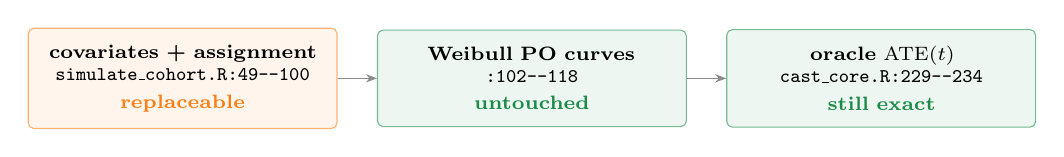
\begin{tikzpicture}[node distance=0.5cm, every node/.style={font=\scriptsize}]
    \node[draw=navorange!60, fill=navorange!8, rounded corners=2pt, text width=3.5cm,
          align=center, inner sep=6pt] (a)
      {\textbf{covariates + assignment}\\ \texttt{simulate\_cohort.R:49--100}\\[2pt]
       \color{navorange}\textbf{replaceable}};
    \node[draw=resultgreen!60, fill=resultgreen!8, rounded corners=2pt, text width=3.5cm,
          align=center, inner sep=6pt, right=of a] (b)
      {\textbf{Weibull PO curves}\\ \texttt{:102--118}\\[2pt]
       \color{resultgreen}\textbf{untouched}};
    \node[draw=resultgreen!60, fill=resultgreen!8, rounded corners=2pt, text width=3.5cm,
          align=center, inner sep=6pt, right=of b] (c)
      {\textbf{oracle} $\mathrm{ATE}(t)$\\ \texttt{cast\_core.R:229--234}\\[2pt]
       \color{resultgreen}\textbf{still exact}};
    \draw[-{Stealth[length=4pt]}, black!45] (a)--(b);
    \draw[-{Stealth[length=4pt]}, black!45] (b)--(c);
  \end{tikzpicture}
  \end{center}

  \vspace{0.5em}
  \textbf{Why the oracle survives.} \texttt{true\_survprob\_ate()} computes $\tau(t)$ by
  averaging $S_1 - S_0$ \emph{over the covariate sample}. It never assumes the
  covariates came from a known parametric law --- only that the potential-outcome
  curves are known for each row.

  \vspace{0.4em}
  \textcolor{accent}{\textbf{So a semi-synthetic covariate sample still yields an
  exactly computable oracle.}} That is what makes this viable rather than merely appealing.
\end{frame}

% ----------------------------------------
\begin{frame}{The honest limit}
  \small
  If we anchor covariates on a real cohort, the survival mechanism --- the linear
  predictor \texttt{lp\_surv} and the treatment model --- is \textbf{still a
  hand-specified function} of those covariates.

  \vspace{0.6em}
  Realism is bought for $p(X, W)$. It is not bought for the outcome model.

  \vspace{0.6em}
  This must be stated in the pilot's README if that work ships. Otherwise the pilot
  would over-claim in precisely the way this dev log spent Part II faulting the app for.

  \vspace{0.6em}
  \textbf{And one more, for the same reason:} the pilot's data note currently reads
  \textit{``All cohorts are simulated from a known generative model. No patient data
  are used or distributed.''} That sentence becomes false the moment a real cohort is
  touched --- and must be rewritten \emph{before}, not after.
\end{frame}

% ========================================
\section{Part V --- Tier 1}
% ========================================

\begin{frame}{Tier 1 --- what we are building}
  \small
  Tier 0 made the app's existing claims true. Tier 1 adds the capability that was
  genuinely missing --- and it is the part that maps onto \texttt{survcausal-pilot}.

  \vspace{0.6em}
  \begin{enumerate}
    \item \textbf{$\tau(X)$ --- heterogeneous effects.} Constant $\tau$ is why Step 4
          cannot currently tell TMLE, AIPW and g-computation apart: they all recover
          the same number. With $\tau(X)$ the comparison acquires teeth.
    \item \textbf{Overlap as its own dial}, separate from $\rho$. Hold $\tau$ and
          confounding fixed, degrade overlap, watch estimators fail.
    \item \textbf{Factorial scenario grid.} Cross
          $\{\text{overlap}\} \times \{\text{confounding}\} \times
          \{\text{heterogeneity}\}$ and summarise in one table --- mirroring
          \texttt{run\_pilot.R}'s design so that one cause moves at a time.
  \end{enumerate}

  \vspace{0.5em}
  \small \textit{All three now built; twelve tests green.}
\end{frame}

% ----------------------------------------
\begin{frame}{$\tau(X)$ --- and the property we designed around}
  \small
  \[
    \tau(X) \;=\; \tau_0 \;+\; \kappa \cdot \sigma_Y \cdot m(X)
  \]

  $m(X)$ is a \emph{centred} covariate index, so $\mathbb{E}[\tau(X)] = \tau_0$.

  \vspace{0.4em}
  \textcolor{accent}{\textbf{Turning heterogeneity on does not move the average
  effect.}} The number the user typed stays the ATE; only the spread changes.

  \vspace{0.4em}
  That is deliberate. Without it, a participant raising $\kappa$ would watch the ATE
  drift and could not tell whether the estimator had broken or the target had simply
  moved --- the same attribution principle as the two seeds, and as the factorial.

  \vspace{0.3em}
  {\footnotesize Measured: $\kappa=0$ gives ATE $-5.000$, sd$(\tau)=0.000$;
  $\kappa=1$ gives ATE $-5.000$, sd$(\tau)=0.852$.}

  \payoff{This is the pilot's named v2 gap. \texttt{survcausal-pilot}'s vignette
  concedes twice that its cohort has no covariate-driven effect modification;
  prototyping it here costs seconds per run instead of ninety minutes.}
\end{frame}

% ----------------------------------------
\begin{frame}{Why constant $\tau$ was holding the app back}
  \small
  With a constant effect, g-computation, IPW, AIPW and TMLE all recover the
  \emph{same number}. A participant comparing them learns only that they agree ---
  the problem is not hard enough to separate them.

  \vspace{0.4em}
  It also makes the clinically important question unaskable:
  \emph{does this work?} versus \emph{does this work \textbf{for this patient}?}
  Only the second requires $\tau$ to vary.

  \vspace{0.4em}
  With $\tau(X)$ live there is finally something for a CATE estimator to find. An
  interacted outcome model recovers the per-patient effect at
  $r = \mathbf{1.000}$ on our own DGP --- which is the right answer, since that model
  is correctly specified here. The interesting version of this question starts when
  it is not.

  \payoff{This is the same quantity the pilot's risk/benefit quadrants are built
  from. The pilot can already \emph{estimate} a CATE; what it lacks is a DGP where
  the true CATE varies.}
\end{frame}

% ----------------------------------------
\begin{frame}{The overlap dial --- and the trade it forces}
  \small
  \begin{columns}[T,totalwidth=\textwidth]
    \begin{column}{0.47\textwidth}
      \textbf{Learned} (Tier 0)\\
      draw $Z$, then $X \mid Z$
      \begin{itemize}
        \item confounding inherited from real data
        \item realistic
        \item \textcolor{navorange}{not adjustable}
      \end{itemize}
    \end{column}
    \begin{column}{0.47\textwidth}
      \textbf{Designed} (Tier 1)\\
      draw $X$, then $Z \mid X$
      \begin{itemize}
        \item $\text{logit}\,e = \alpha + \lambda m(X) + \rho U$
        \item \textcolor{resultgreen}{$\lambda$ is a dial}
        \item arm structure is ours, not the data's
      \end{itemize}
    \end{column}
  \end{columns}

  \vspace{0.6em}
  \textbf{You cannot have both from a conditional VAE.} $p(X \mid Z)$ and a
  controllable $e(X)$ pull in opposite directions.

  \vspace{0.4em}
  \textcolor{accent}{\textbf{Getting realistic covariates \emph{and} a designed
  propensity out of one model is exactly what CausalMix's overlap regulariser is
  for}} --- the second concrete, measured argument for Tier 2.
\end{frame}

% ----------------------------------------
\begin{frame}{What $\lambda$ actually does}
  \small
  \begin{center}
  \footnotesize
  \begin{tabular}{@{}llrl@{}}
    \toprule
    $\lambda$ & \textbf{propensity range} & \textbf{\% extreme} & \textbf{reading} \\
    \midrule
    $0$ & $[0.565,\ 0.565]$ & $0.0\%$  & randomised trial on realistic covariates \\
    $1$ & $[0.136,\ 0.895]$ & $0.0\%$  & real confounding, comfortable overlap \\
    $3$ & $[0.003,\ 0.999]$ & $33.6\%$ & confounding \emph{and} positivity failure \\
    \bottomrule
  \end{tabular}
  \end{center}

  \vspace{0.5em}
  Note the middle row. \textbf{Confounding and positivity are separate failures.} At
  $\lambda = 1$ the naive estimate is badly biased ($+0.68$) while every propensity
  stays comfortably interior --- exactly the setting where adjustment is supposed to
  work, and does.

  \vspace{0.4em}
  A dial that conflated the two would teach the wrong lesson. This one does not, and
  the test suite asserts that it does not.

  \payoff{Positivity is a first-class identification assumption in Modules C and D.
  Until now no teaching asset let anyone \emph{move} it.}
\end{frame}

% ----------------------------------------
\begin{frame}{The factorial grid}
  \small
  Three axes crossed, everything else held fixed --- generator, covariates, $\tau_0$,
  $n$. Twelve cells. Selected rows:

  \begin{center}
  \scriptsize
  \begin{tabular}{@{}lllrrr@{}}
    \toprule
    \textbf{overlap} & \textbf{effect} & \textbf{hidden} & \textbf{naive bias} &
    \textbf{g-comp bias} & \textbf{\% extreme} \\
    \midrule
    randomised & constant & none    & $-0.013$ & $-0.030$ & $0.0\%$ \\
    randomised & varies   & none    & $-0.086$ & $-0.047$ & $0.0\%$ \\
    mild       & constant & none    & $+0.684$ & $-0.042$ & $0.0\%$ \\
    mild       & varies   & present & $+0.994$ & $+0.072$ & $0.2\%$ \\
    poor       & constant & none    & $+1.166$ & $+0.037$ & $33.6\%$ \\
    poor       & varies   & present & $+1.900$ & $+0.080$ & $35.3\%$ \\
    \bottomrule
  \end{tabular}
  \end{center}

  \vspace{0.4em}
  Each axis moves something the others do not --- positivity tracks $\lambda$ alone,
  effect spread tracks $\kappa$ alone, residual-bias-after-adjustment tracks $\rho$
  alone. \textbf{That separation is asserted by the test suite}, because a factorial
  whose axes move together is not a factorial.

  \payoff{Directly mirrors \texttt{run\_pilot.R}'s 2$\times$2 at fixed effect size.
  Same discipline, three axes instead of two, seconds instead of hours.}
\end{frame}

% ----------------------------------------
\begin{frame}{A limitation the grid exposed}
  \small
  Building the dial surfaced something about the generator.

  \vspace{0.5em}
  The prognostic index has \textbf{unit} standard deviation on real training data by
  construction. On synthetic covariates it comes out at $\mathbf{0.852}$.

  \vspace{0.5em}
  The CVAE, trained with a squared-error reconstruction loss, systematically
  \textbf{shrinks variance} --- visible too in the raw ranges: real age spans
  $[7,\ 116]$, synthetic $[36,\ 98]$.

  \vspace{0.4em}
  Practical consequence: the overlap dial runs about \textbf{15\% weak} ---
  $\lambda = 3$ behaves like roughly $\lambda = 2.6$. This is now a tripwire test
  rather than a footnote: if the ratio collapses further, the grid's axis labels
  stop meaning what they say.

  \payoff{Third measured argument for Tier 2: a mixture-of-Gaussians prior exists
  precisely to stop a single-Gaussian latent from collapsing the spread of the data
  it is modelling.}
\end{frame}

% ----------------------------------------
\begin{frame}{Where Tier 1 leaves us}
  \small
  \begin{columns}[T,totalwidth=\textwidth]
    \begin{column}{0.47\textwidth}
      \textbf{The app can now}
      \begin{itemize}
        \item vary the effect across patients
        \item dial positivity independently of confounding
        \item run a 12-cell attributable factorial
        \item score two estimators against known truth in every cell
      \end{itemize}
    \end{column}
    \begin{column}{0.47\textwidth}
      \textbf{Three measured arguments for Tier 2}
      \begin{enumerate}
        \item typed decoders --- defect 10
        \item overlap regulariser --- the trade on the previous slide
        \item mixture prior --- variance shrinkage
      \end{enumerate}
    \end{column}
  \end{columns}

  \vspace{0.5em}
  None of these three was an appeal to authority. Each came out of a number we
  watched go wrong.

  \vspace{0.3em}
  \textcolor{accent}{\textbf{Next:}} Tier 2 puts the generator behind an interface and
  ships pre-fit artifacts; Tier 3 is the \texttt{survcausal-pilot} integration ---
  real covariates, oracle $\mathrm{ATE}(t)$ intact.
\end{frame}

% ----------------------------------------
\begin{frame}{References}
  \small
  \begin{itemize}
    \item Parikh H, Vajao C, Xu L, Tchetgen Tchetgen E (2022).
          \emph{Validating Causal Inference Methods}. ICML (PMLR 162).
          \url{https://arxiv.org/abs/2202.04208}
    \item Zhang Q, Parikh H, Naimi A, Nabi R, Kim C, Lash T (2026).
          \emph{CausalMix: Controllable Generative Sandbox for Causal Inference}.
          \url{https://arxiv.org/abs/2603.03587}
    \item Yang E, et al., Shuryak I (2025). \emph{CAST: Time-Varying Treatment Effects}.
          \url{https://arxiv.org/abs/2505.06367}
    \item Shamsutdinova D, Shuryak I, Yang E. \texttt{survcausal-pilot}.
          \url{https://github.com/ishuryak/survcausal-pilot}
    \item Kingma DP, Welling M (2014). \emph{Auto-Encoding Variational Bayes}. ICLR.
    \item Dang LE, Balzer LB (2023). \emph{Start with the Target Trial Protocol, Then
          Follow the Roadmap for Causal Inference}. Epidemiology 34(5):619--623.
  \end{itemize}
\end{frame}

\end{document}
